\documentclass[12pt,a4paper]{scrartcl}
%\usepackage[utf8]{inputenc} хз не влияет
\usepackage[english,russian]{babel}
\usepackage[T2A]{fontenc} 
%\usepackage{kurier}
\usepackage{setspace}
\usepackage[left=5mm,right=5mm, top=3mm,bottom=3mm,bindingoffset=0cm]{geometry}
\usepackage{graphicx}
\usepackage{multicol}
\usepackage{amsmath}
\usepackage{amssymb}
\usepackage{array}

\pagenumbering{gobble}

\begin{document}
%	\pagestyle{colontituls}

	\begin{center}
		%{\fontfamily{kurier}рвиа 6} каким-то образом поменять шрифт
		\Large{6}
	\end{center}
	
	\vspace{-8mm}
	\noindent\rule{\textwidth}{0,5pt}
	\begin{center}
		\vspace{-3mm}
		\tiny{АЛЕКСАНДР МИХАЙЛОВ}
	\end{center}

	\begin{table}[h]
		\begin{tabular}{rl}
			
			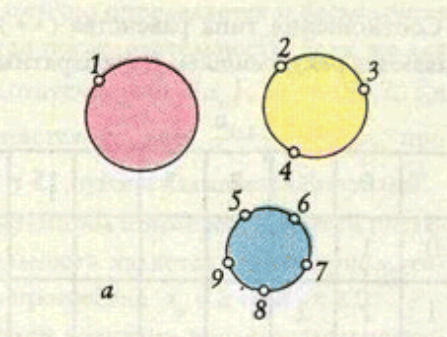
\includegraphics{page1.png} & 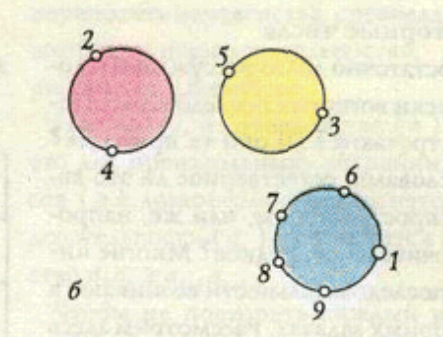
\includegraphics{page2.png} \\
			
		\end{tabular}
	\end{table}

	\vspace{-10mm}
	\begin{center}
		\textsl{\footnotesize{Рисунок 2.}}
		\textit{\footnotesize{К определению $s_{\vec{\mu}}(u,v)$.}}
	\end{center}

	\begin{multicols}{2}
		лить на~$m-1$ групп (с~указанием в~каждой \\ группе, кто за кем следует по~кругу). Дру\-гих вариантов имеется $(n-1)s(n-1,m)$, поскольку каждое такое расположение можно получить следующим способом: разбить остальных участников на $m$ групп, рассадить их за столами, а затем указать вам, за кем вы следуете, т.е. посадить вас на какое-либо место за один из столов. На рисунке $2,a$ вы в гордом одиночестве сидите за первым столом. На рисунке $2,$\textit{б} 8 человек уже сидят за тремя столами, и вас направляют за третий стол --- между 6-м и 9-м учениками.
		
		Итак, доказано равенство
		\vspace{-3mm}
		\[
			s(n,m)=s(n-1,m-1)+(n-1)s(n-1,m)
		\]
		при $n\geqslant1$. Будем считать, что $s(0,0)=1,$--- это согласуется со значением $s(1,1)=1$. <<Неправильные>> члены опять удобно считать равными 0. Кроме того,
		\renewcommand{\arraystretch}{1.8} %% increase table row spacing
		\renewcommand{\tabcolsep}{5mm} %% increase table column spacing
		\begin{center}
			\begin{tabular}{*{7}{|c}|}
				\hline
				& 0 & 1 & 2 & 3 & 4 & 5 \\
				\hline
				0 & 1 &   &   &   &   &   \\
				\hline
				1 & 0 & 1 &   &   &   &   \\
				\hline
				2 & 0 & 1 & 1 &   &   &   \\
				\hline
				3 & 0 & 2 & 3 & 1 &   &   \\
				\hline
				4 & 0 & 6 & 11 & 6 & 1 &  \\
				\hline
				5 & 0 & 24 & 50 & 35 & 10 & 1 \\
				\hline
			\end{tabular}
			
			\textsl{\footnotesize{Таблица 2}}
		\end{center}
			
		$s(n,m)=1$ при $m-n\geqslant0$. Все это позволяет создать таблицу 2.
		
		Даже гипотетически приятно считать, что вы попали в группу отъезжающих в Америку, не так ли? Ну, а теперь предположим, что Вам повезло и вы в Шереметьеве-2 стоите в очереди на таможенный досмотр. Очередь тянется долго,и чтобы занять время, вы подсчитываете число таких случаев в вашей группе, когда менее высокий человек стоит ближе к цели, чем высокий. Сколькими способами можно построить $m$ человек разного роста в одну шеренгу так, чтобы имелось ровно $k$ таких пар, в которых менее высокий стоит левее более высокого? Обозначим это число $M(m,k).$ (Оно называется числом Мак-Магона.)
		
		Заметим, что если самого высокого из группы послать за мороженым, то в оставшейся группе число пар, в которых менее высокий стоит перед более высоким, уменьшится на $i-1$, где $i$ --- номер места в очереди этого <<самого высокого>>. Отсюда следует равенство
		\begin{gather*}
			M(m,k)=M(m-1,k)+M(m-1,k-1)+\ldots \\
			 \ldots+m(m-1,k-m+1)   
		\end{gather*}
		--- здесь, как и прежде, $m\geqslant1$ и $i$-е слагаемое отвечает случаю, когда <<самый высокий>> стоял на $i$-м месте. Опять договоримся об обращении в 0 <<неправильных>> членов. Скажем, будем считать, что $M(0,0)=1$. Снова составим таблицу (таблица 3).
		
	\end{multicols}	

		
\end{document}